\Chapter{Grafikus szerkesztőeszköz}

\section{Az editor funkciói}

\begin{itemize}
\item Admin felület: Ennek a grafikus felületnek az a célja, hogy az
adatbázissal kapcsolatos műveleteket grafikus felületen kezelhessük, nem pedig konzolos parancsok beírásával.
\item Térkép szerkesztő: Grafikus felületen összerakhatjuk a játékban szereplő térképet, és a háttérben ezeket a lekérdezéseket az editor adja ki.
\item Debug eszköz: Beírhatunk lekérdezéseket is a szerkesztőbe, és a lekérdezés eredményét rögtön láthatjuk is a térképen. Ha elemek kijelölése volt a lekérdezésben, akkor a térképen piros keretet rak az eredményhalmazban szereplő entitások köré.
	
\end{itemize}

\section{Implementáció}

A grafikus szerkesztőeszközt is Java nyelven implementáltam. Itt a szerkesztő az adatbázismotort könyvtárként foglalja magába. Az editor az egy egyszerű Swinges alkalmazásként lett megvalósítva. 

\section{Editor használati útmutató}

\begin{figure}[htb]
	\begin{center}
		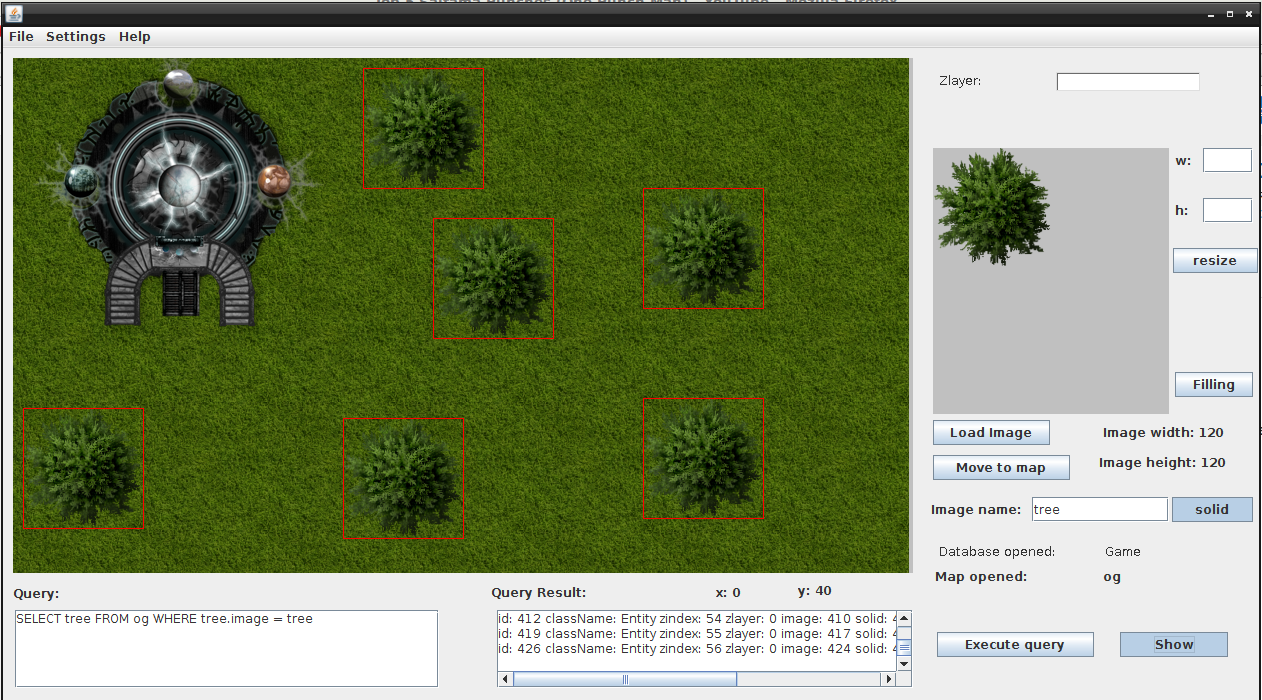
\includegraphics[scale=0.3]{images/editor}
		\caption{A Tile Editor használat közben}
		\label{fig:editor}
	\end{center}
\end{figure}

A File menü alatt hozható létre új adatbázis, azon belül új map, illetve létező adatbázis, és map is innen érhető el. Ez a menüpont tartalmaz még egy Save opciót is, ami arra szolgál, hogy a változtatásokat mentsük a JSOn fájlba. Ha módosítunk az adatbázison, de a Save menüt nem használjuk, akkor az editor kikapcsolása után a memóriából az összes változtatás eltűnik, és perzsiztens állapotról így nem gondoskodik.

Settings menü egyetlen funkciót tartalmaz, a Camera Settings beállítást, ami arra szolgál, hogy az irányító gombokkal(fel,le,jobbra,balra) hány pixelt ugorjon a kamera. Az alapértelmezett beállítás az, hogy az y tengely és az x tengely irányába is 10 pixellel mozdul el.
Ez azért fontos, mert nem lehet egérrel képeket beszúrni, hanem a "Move to Map" gombra kattintva szúr be egy képet a térképből látható terület bal felső sarkához igazítva. 

A Help menü alatt található egy rövid használati útmutató az alkalmazáshoz.

A főablak legnagyobb részét a térkép teszi ki, ahová beilleszthetünk képeket. Mellette a zlayer szövegdoboz arra szolgál, hogy egy számot írjunk bele, aminek akkor van jelentősége, amikor egy képet szúrunk a térképre, ugyanis ez a háttérben lefutó insert lekérdezésben a LAYER kulcsszó után szereplő attribútum. Ha ezt a mezőt nem töltjük ki, akkor sincs semmi probléma, olyankor a lekérdezés a háttérben automatikusan 0 értéket vesz fel a zlayernek.

A nagy térkép mellett látható egy kisebb téglalap is, amiben képek jelenhetnek meg. Ennek az a funkciója, hogy a beszúrandó képeket láthatjuk ott, illetve a mellette lévő két szövegdobozban(w, h) átméretezhetjük azt. 

A LoadImage gomb segítségével érhetjük el a fájlrendszert, és tölthetünk be onnan képet az imént említett dobozba.

Az ImageWidth és ImageHeight feliratok az aktuálisan betöltött kép attribútumai, ez az információ hasznos lehet, mert így a kamerát beállíthatjuk, hogy milyen mértékben mozduljon el felhasználói beavatkozásra, és a betöltött képet kényelmesebben szúrhatjuk be.

Ha a "Move to Map" gombra kattintunk, viszont az "Image Name" szövegdobozba nem adtuk meg a beszúrandó kép nevét, akkor az alkalmazás figyelmeztetni fog, hogy ezt tegyük meg. Amit abba a szövegdobozba írunk, az a beszúrandó Entity objektum image attribútumának lesz az értéke. 

A "solid" az egy JToogleButton, ami azt jelenti, hogy két állapota van, vagy lenyomva van, vagy alapértelmezetten. Ha nincs aktiválva, akkor a beszúrandó új Entity objektum solid attribútumának értéke false lesz, ha aktiválva van akkor true. Ez azért fontos mert az ütközésvizsgálat ezen attribútumra épül, ugyanis ha egy entitás nem solid, akkor az ütközésvizsgálat szempontjából semleges.

Az "Image Name" szövegdoboz alatt két felirat látható, amelyek az épp aktuálisan megnyitott adatbázis és map nevét mutatják. Ha megnyitjuk az editort akkor ezek értelem szerűen még nem tartalmaznak értéket, ezért ilyenkor a "-" karakter látható feltüntetve.

Az "Execute Query" gombra kattintva a "Query" Szövegmezőben látható lekérdezés fog lefutni, aminek eredménye a "Query Result:" szövegmezőben látható. Ha bekapcsolja a felhasználó a debug módot, akkor e térképen a lekérdezés eredményei láthatóvá válnak oly módon, hogy egy piros taglalap rajzolódik köré. A debig módot a show JToogleButton aktiválásával lehet bekapcsolni. 

